% =====================================================================
% Section 4: Setup & Reproduction
% "Stealthy Computational Delay Attacks on Control Systems"
% (Nauta, Sandberg, Maggio, ICCPS 2025)
% Beamer, Madrid theme, green, 9pt, 16:9
% Compile: pdflatex main.tex (twice)   or   latexmk -pdf main.tex
% =====================================================================
\documentclass[9pt,aspectratio=169]{beamer}
% \setbeameroption{show notes on second screen=right}   % uncomment to see speaker notes

\usetheme{Madrid}
\usepackage[T1]{fontenc}
\usepackage[utf8]{inputenc}
\usepackage{amsmath,amssymb}
\usepackage{tikz}
\usetikzlibrary{arrows.meta,positioning,shapes.geometric,shapes.symbols,calc,fit}
\usepackage{pgfplots}
\pgfplotsset{compat=1.18}
\usepackage{tabularx,booktabs,colortbl}

% ---------------- green palette ----------------
\definecolor{mgreen}{HTML}{036B3A}   % main green
\definecolor{mgreenD}{HTML}{02502B}  % dark green
\definecolor{mgreenM}{HTML}{4E9A6E}  % mid green
\definecolor{mgreenL}{HTML}{E3F1E8}  % light green fill
\definecolor{mgreenXL}{HTML}{F2F8F4} % very light fill
\definecolor{accent}{HTML}{B4521C}   % orange accent (highlights, rejections)
\definecolor{accentL}{HTML}{F8E6DA}
\definecolor{ink}{HTML}{1C2430}
\definecolor{body}{HTML}{4A5260}
\definecolor{rulec}{HTML}{C9D6CE}

\setbeamercolor{structure}{fg=mgreen}
\setbeamercolor{palette primary}{bg=mgreen,fg=white}
\setbeamercolor{palette secondary}{bg=mgreenD!80!mgreen,fg=white}
\setbeamercolor{palette tertiary}{bg=mgreenD,fg=white}
\setbeamercolor{palette quaternary}{bg=mgreenD,fg=white}
\setbeamercolor{frametitle}{bg=mgreen,fg=white}
\setbeamercolor{framesubtitle}{fg=mgreenL}
\setbeamercolor{title}{bg=mgreen,fg=white}
\setbeamercolor{block title}{bg=mgreen,fg=white}
\setbeamercolor{block body}{bg=mgreenL,fg=ink}
\setbeamercolor{block title alerted}{bg=accent,fg=white}
\setbeamercolor{block body alerted}{bg=accentL,fg=ink}
\setbeamercolor{item}{fg=mgreen}
\setbeamercolor{normal text}{fg=ink}
\setbeamertemplate{navigation symbols}{}
\setbeamertemplate{itemize items}[circle]
\setbeamerfont{block title}{size=\scriptsize}
\setbeamerfont{block body}{size=\scriptsize}
\setbeamerfont{block title alerted}{size=\scriptsize}
\setbeamerfont{block body alerted}{size=\scriptsize}

\title[Setup \& Reproduction]{Stealthy Computational Delay Attacks on Control Systems}
\subtitle{Section 4: Setup \& Reproduction}
\author[Section 4]{[Your name]}
\institute[CS637]{CS637 \textperiodcentered{} Paper \& code presentation}
\date[ICCPS 2025]{Nauta, Sandberg \& Maggio, ICCPS 2025}

% ---------------- helpers ----------------
\newcommand{\abar}{\ensuremath{\bar a}}
\newcommand{\phatm}{\ensuremath{\hat p_{\mathrm m}}}
\newcommand{\takeaway}[1]{{\small\color{mgreenD}\itshape #1\par}\vspace{1.2ex}}
\newcommand{\code}[1]{{\ttfamily #1}}

\tikzset{
  >={Latex[length=1.8mm]},
  arr/.style={->, thick, mgreenD},
  stage/.style={draw=mgreen, fill=mgreen, text=white, rounded corners=2pt, font=\scriptsize\bfseries,
                minimum height=0.62cm, text width=2.6cm, align=center},
  detail/.style={draw=rulec, fill=mgreenXL, rounded corners=2pt, font=\tiny, text width=2.6cm,
                 align=left, inner sep=1.5mm},
  box/.style={draw=mgreen, thick, fill=mgreenXL, rounded corners=2pt, font=\scriptsize, align=left, inner sep=1.6mm},
  darkbox/.style={draw=mgreenD, fill=mgreenD, text=white, rounded corners=2pt, font=\scriptsize, align=left, inner sep=1.6mm},
  dec/.style={diamond, aspect=1.9, draw=mgreen, thick, fill=mgreenL, font=\tiny, align=center, inner sep=0.4mm},
  reject/.style={draw=accent, fill=accentL, rounded corners=2pt, font=\tiny, align=center, inner sep=1.2mm, text width=2.3cm},
  pill/.style={draw=mgreen, fill=mgreenL, rounded corners=6pt, font=\tiny\bfseries, inner sep=1.4mm, align=center},
}

\begin{document}

% =====================================================================
% 1. Section cover with roadmap
% =====================================================================
\begin{frame}
\note{Section 4 is Setup and Reproduction: the authors' code and our reimplementation. The roadmap shows where we are in the group talk. Inside this section there are three parts. Part 1, the authors' structure: how the repeatability package is organised into drivers, solvers, results and plots. Part 2, all related cases: the nine combinations of plant and detector, which figure each one produces, and why we zoom in on main\_short.py. Part 3, the code itself: a flowchart of main\_short.py, one solver call worked through as a decision flow, and the full output, which we reproduced without Gurobi and compared with the paper's Figure 2.}
\vspace{0.2cm}
\begin{center}
{\scriptsize\bfseries\color{accent} SECTION 4}\\[0.25cm]
{\LARGE\bfseries\color{mgreen} Setup \& Reproduction}\\[0.2cm]
{\small\itshape\color{body} The authors' code, every case it runs, and our reimplementation of its reduced experiment}
\end{center}
\vspace{0.25cm}

% --- group roadmap ---
\begin{center}
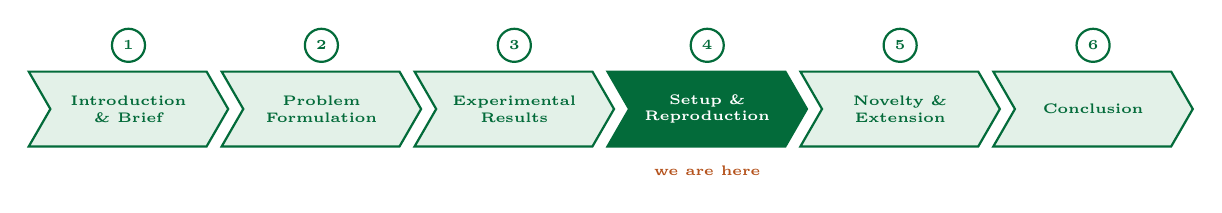
\begin{tikzpicture}[
  chev/.style={signal, signal to=east, signal from=west, signal pointer angle=120, draw=mgreen, thick,
               minimum height=0.95cm, minimum width=2.45cm, text width=1.75cm, align=center, font=\tiny\bfseries},
]
\foreach \i/\t/\x in {1/{Introduction\\\& Brief}/0, 2/{Problem\\Formulation}/2.45, 3/{Experimental\\Results}/4.9,
                      4/{Setup \&\\Reproduction}/7.35, 5/{Novelty \&\\Extension}/9.8, 6/{Conclusion}/12.25}{
  \ifnum\i=4
    \node[chev, fill=mgreen, text=white] (c\i) at (\x,0) {\t};
  \else
    \node[chev, fill=mgreenL, text=mgreen] (c\i) at (\x,0) {\t};
  \fi
  \node[circle, draw=mgreen, thick, fill=white, font=\tiny\bfseries, text=mgreen, inner sep=1pt, minimum size=0.42cm]
       at ($(c\i.north)+(0,0.32)$) {\i};
}
\node[font=\tiny\bfseries, text=accent] at ($(c4.south)+(0,-0.3)$) {we are here};
\end{tikzpicture}
\end{center}
\vspace{0.15cm}

% --- three parts of this section ---
\begin{center}
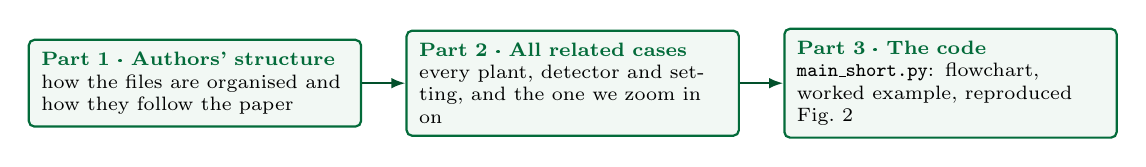
\begin{tikzpicture}[node distance=0.55cm]
\node[box, text width=3.9cm] (p1) {\textbf{\color{mgreen}Part 1 \textperiodcentered{} Authors' structure}\\ how the files are organised and how they follow the paper};
\node[box, text width=3.9cm, right=of p1] (p2) {\textbf{\color{mgreen}Part 2 \textperiodcentered{} All related cases}\\ every plant, detector and setting, and the one we zoom in on};
\node[box, text width=3.9cm, right=of p2] (p3) {\textbf{\color{mgreen}Part 3 \textperiodcentered{} The code}\\ \code{main\_short.py}: flowchart, worked example, reproduced Fig.~2};
\draw[arr] (p1) -- (p2); \draw[arr] (p2) -- (p3);
\end{tikzpicture}
\end{center}
\vfill
{\tiny\color{body} Source: Nauta, Sandberg \& Maggio, ICCPS 2025 \textperiodcentered{} REP code: doi.org/10.5281/zenodo.14792914 \textperiodcentered{} DOI 10.1145/3716550.3722013}
\end{frame}

% =====================================================================
% 2. Part 1: authors' structure (pipeline diagram)
% =====================================================================
\begin{frame}{How the authors organised the code}{Part 1 \textperiodcentered{} Authors' structure}
\note{The package is a flat pipeline of four layers, read left to right. Drivers: main.py runs everything, main\_short.py is a quick reduced run, main\_fig2, 3 and 4 each regenerate one figure. All share define\_system, which holds the hard-coded closed-loop matrices for each plant, and nested loops that pick each case (paper Sections 3 and 5.1). For every case the driver calls the solver with exec, so the loop variables reach it as globals. Solvers: one script per detector, binomial only, chi-square only, or both; each builds one mixed-integer optimisation and solves it with Gurobi (Section 4, Eqs 4 to 11). Results: every case appends rows to a CSV and a TXT whose folder and file name encode the case, one row per attack length. Plots: pgfplots files read the CSVs and draw Figures 2 to 4 (Section 5.4). Design choices at the bottom: one driver per figure, one solver per detector with the combined one a superset, exec instead of functions, and file names that encode the configuration.}
\takeaway{Four layers, run left to right: a driver picks a case, a solver finds the worst attack, the results are saved, and plots draw the paper's figures.}

\begin{center}
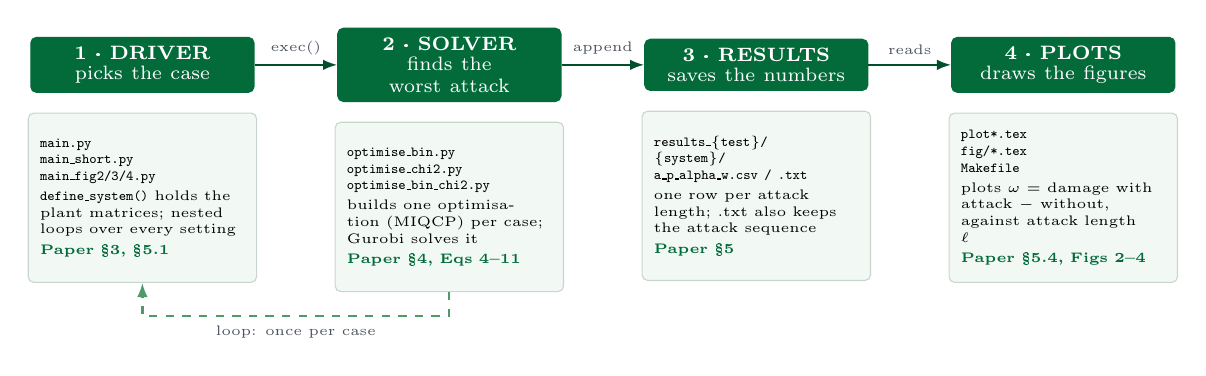
\begin{tikzpicture}[node distance=1.05cm]
\node[stage] (s1) {1 \textperiodcentered{} DRIVER\\[-1pt]{\normalfont picks the case}};
\node[stage, right=of s1] (s2) {2 \textperiodcentered{} SOLVER\\[-1pt]{\normalfont finds the worst attack}};
\node[stage, right=of s2] (s3) {3 \textperiodcentered{} RESULTS\\[-1pt]{\normalfont saves the numbers}};
\node[stage, right=of s3] (s4) {4 \textperiodcentered{} PLOTS\\[-1pt]{\normalfont draws the figures}};
\draw[arr] (s1) -- node[above, font=\tiny, text=body]{exec()} (s2);
\draw[arr] (s2) -- node[above, font=\tiny, text=body]{append} (s3);
\draw[arr] (s3) -- node[above, font=\tiny, text=body]{reads} (s4);

\node[detail, below=0.25cm of s1, minimum height=2.15cm, anchor=north] (d1)
  {\code{main.py}\\\code{main\_short.py}\\\code{main\_fig2/3/4.py}\\[0.6ex]
   \code{define\_system()} holds the plant matrices; nested loops over every setting\\[0.6ex]
   {\color{mgreen}\bfseries Paper \S3, \S5.1}};
\node[detail, below=0.25cm of s2, minimum height=2.15cm, anchor=north] (d2)
  {\code{optimise\_bin.py}\\\code{optimise\_chi2.py}\\\code{optimise\_bin\_chi2.py}\\[0.6ex]
   builds one optimisation (MIQCP) per case; Gurobi solves it\\[0.6ex]
   {\color{mgreen}\bfseries Paper \S4, Eqs 4--11}};
\node[detail, below=0.25cm of s3, minimum height=2.15cm, anchor=north] (d3)
  {\code{results\_\{test\}/}\\\code{\{system\}/}\\\code{a\_p\_alpha\_w.csv / .txt}\\[0.6ex]
   one row per attack length; .txt also keeps the attack sequence\\[0.6ex]
   {\color{mgreen}\bfseries Paper \S5}};
\node[detail, below=0.25cm of s4, minimum height=2.15cm, anchor=north] (d4)
  {\code{plot*.tex}\\\code{fig/*.tex}\\\code{Makefile}\\[0.6ex]
   plots $\omega$ = damage with attack $-$ without, against attack length $\ell$\\[0.6ex]
   {\color{mgreen}\bfseries Paper \S5.4, Figs 2--4}};

\draw[arr, mgreenM, dashed] (d2.south) -- ++(0,-0.3) -| node[pos=0.25, below, font=\tiny, text=body]{loop: once per case} (d1.south);
\end{tikzpicture}
\end{center}

\vspace{-0.1cm}
\begin{columns}[T,onlytextwidth]
\begin{column}{0.24\textwidth}\begin{block}{One driver per figure}same code, only the loop values change\end{block}\end{column}
\begin{column}{0.24\textwidth}\begin{block}{One solver per detector}\code{bin\_chi2} = both tests together\end{block}\end{column}
\begin{column}{0.24\textwidth}\begin{block}{Linked by exec()}loop settings reach the solver as globals\end{block}\end{column}
\begin{column}{0.24\textwidth}\begin{block}{File name = the case}\code{a3\_p0.25\_alpha0.01\_w20} $\to$ \abar, \phatm, $\alpha$, $n_w$\end{block}\end{column}
\end{columns}
\end{frame}

% =====================================================================
% 3. Part 2: all related cases (matrix + driver-to-figure map)
% =====================================================================
\begin{frame}{Every case the code can run, and our focus}{Part 2 \textperiodcentered{} All related cases}
\note{A case is a plant configuration times a detector. The pendulum is open-loop unstable and was also run on real hardware; it appears with the zero policy (motor gets zero on a missed deadline) and the hold policy (keeps its last value). The quadruple tank is open-loop stable and non-minimum phase and uses hold. Detectors: binomial only, chi-square only, or both; the watchdog is always on. That gives nine cases; each cell says which figure or table uses it; hold with chi-square and hold with both are computed only by main.py. The diagram shows which driver produces which output and what it fixes: main.py sweeps everything, main\_fig2 fixes window 20 and varies the watchdog limit 1 to 4, main\_fig3 fixes a-bar 4 and window 20 to compare detectors, main\_fig4 fixes a-bar 4 and varies the window 10 to 18, and main\_short fixes one case. Special cases: window longer than the attack gives a single binomial constraint; chi-square only ignores the window so it runs once at 20; first and last slots are forced hits so 27 slots give lengths 1 to 25; the tank's output is half its level so plots divide omega by 4. Our focus is the highlighted cell: 27 solves instead of 68,445, about 2 hours instead of weeks, same solver code; the authors use it as their environment test (Appendix A.4.1).}
\vspace{-0.6ex}\takeaway{A case = a plant setup $\times$ a detector: $3\times3=9$ cases. Each cell shows which paper figure it produces.}

{\scriptsize
\renewcommand{\arraystretch}{1.1}
\noindent\begin{tabularx}{\linewidth}{>{\raggedright}p{4.4cm}XXX}
\rowcolor{mgreen}\color{white}\textbf{Plant setup $\downarrow$ \textperiodcentered{} Detector $\to$} & \color{white}\textbf{Binomial only} & \color{white}\textbf{$\chi^2$ only} & \color{white}\textbf{Binomial + $\chi^2$}\\
\rowcolor{accentL}\textbf{furuta\_zero}: pendulum (unstable), zero & Fig 3, Fig 4 & Fig 3 & Fig 2, Fig 3 \textperiodcentered{} \textbf{\color{accent}our focus}\\
\rowcolor{mgreenXL}\textbf{furuta\_hold}: pendulum (unstable), hold & Fig 4, Table 1 & main.py only & main.py only\\
\rowcolor{mgreenL}\textbf{qt\_nmp}: quad tank (stable), hold & Fig 3 & Fig 3 & Fig 2, Fig 3\\
\end{tabularx}}
\vspace{0.5ex}

\begin{columns}[T,onlytextwidth]
\begin{column}{0.6\textwidth}
{\scriptsize\bfseries\color{mgreen} Which driver makes which output, and what it fixes}\\[0.4ex]
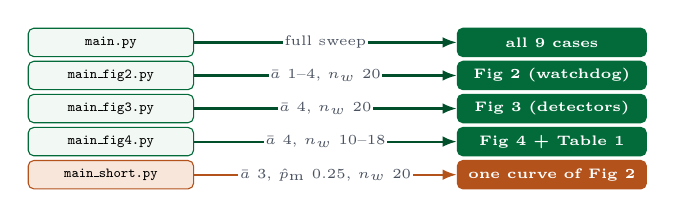
\begin{tikzpicture}[
  drv/.style={draw=mgreen, fill=mgreenXL, rounded corners=2pt, font=\tiny\ttfamily, minimum width=2.1cm, minimum height=0.36cm, inner sep=0.8mm},
  outn/.style={draw=mgreen, fill=mgreen, text=white, rounded corners=2pt, font=\tiny\bfseries, minimum width=2.4cm, minimum height=0.36cm, inner sep=0.8mm},
  lab/.style={font=\tiny, text=body, fill=white, inner sep=0.5pt},
]
\foreach \d/\o/\l/\y in {main.py/{all 9 cases}/{full sweep}/0,
                         main\_fig2.py/{Fig 2 (watchdog)}/{\abar{} 1--4, $n_w$ 20}/-0.42,
                         main\_fig3.py/{Fig 3 (detectors)}/{\abar{} 4, $n_w$ 20}/-0.84,
                         main\_fig4.py/{Fig 4 + Table 1}/{\abar{} 4, $n_w$ 10--18}/-1.26}{
  \node[drv] (dr) at (0,\y) {\d};
  \node[outn] (ou) at (5.6,\y) {\o};
  \draw[arr] (dr) -- node[lab]{\l} (ou);
}
\node[drv, fill=accentL, draw=accent] (ds) at (0,-1.68) {main\_short.py};
\node[outn, fill=accent, draw=accent] (os) at (5.6,-1.68) {one curve of Fig 2};
\draw[arr, accent] (ds) -- node[lab]{\abar{} 3, \phatm{} 0.25, $n_w$ 20} (os);
\end{tikzpicture}\\[0.3ex]
{\tiny\color{body} All figures use \phatm{} = 0.09, 0.17, 0.25 and $\alpha=0.01$.}
\end{column}
\begin{column}{0.37\textwidth}
\begin{block}{Settings swept by main.py}
$\ell$ attack length 1--25 \textperiodcentered{} \abar{} watchdog limit 1--5\\
\phatm{} normal miss rate 0.01--0.25\\
$n_w$ window 10--20 \textperiodcentered{} $\alpha=0.01$
\end{block}
\vspace{-0.5ex}
\begin{alertblock}{Special cases in the code}
Window $\ge$ attack $\to$ one binomial check\\
$\chi^2$-only ignores window $\to$ run once at 20\\
Ends forced on time: $\ell$ = a\_length $-$ 2\\
Tank output = $\tfrac12$ level $\to$ plots $\div$ 4
\end{alertblock}
\end{column}
\end{columns}

\vspace{0.4ex}
\begin{beamercolorbox}[rounded=true, wd=\linewidth, sep=1.2mm]{palette tertiary}
\scriptsize\textbf{OUR FOCUS \textperiodcentered{} main\_short.py} = the highlighted cell: \textbf{27 solves} vs 68,445 in main.py ($\sim$2 h vs weeks), same solver code.
\textit{Why:} pendulum is unstable and real hardware \textperiodcentered{} \abar{} = 3, past which the watchdog stops mattering \textperiodcentered{} \phatm{} = 0.25 gives the clearest effect \textperiodcentered{} bin + $\chi^2$ uses every constraint.
\end{beamercolorbox}
\end{frame}

% =====================================================================
% 4. Part 3: main_short.py flowchart
% =====================================================================
\begin{frame}{How main\_short.py runs, step by step}{Part 3 \textperiodcentered{} The code}
\note{Left: main\_short.py sets alpha 0.01, loads the pendulum with the zero policy from define\_system (the 7 by 7 matrices Phi-h and Phi-m, Q on the angle, the start state), creates the results folder (if it exists it prints already done and carries on, unlike main.py which exits), then loops a\_length from 1 to 27 and runs optimise\_bin\_chi2.py with exec each time. Right: nine steps; steps 5 to 9 are the paper's equations. Step 3: zs are the attack bits, xs the closed-loop states psi = [x; y-tilde; z; u], 3 + 3 + 0 + 1 = 7 numbers, bounded to plus or minus 1000 or Gurobi calls the model unbounded. Step 4: first and last slots are forced hits, so every run of misses is closed by a hit; that is why 27 slots give lengths 1 to 25. Step 5: indicator constraints, z = 0 enforces the hit equation, z = 1 the miss equation; for the zero policy the last row of Phi-miss is zero. Step 6: any 4 slots hold at most 3 misses. Step 7: binom.ppf(0.99, 20, 0.25) = 10. Step 8, the chi-square trick: aux = (1 - z\_i) + the k middle bits + (1 - z\_(i+k+1)) - (k+1) equals 1 only for hit, k misses, hit; max(aux, 0) counts runs m\_k; N = sum of m\_k; expected p\_k N with p\_k = 0.75, 0.19, 0.05, 0.02; since N is a variable the critical value 11.34 is multiplied by N instead of dividing. Step 9: maximise xs[L-1]' Q xs[L-1] and append the best row.}
\takeaway{The driver tries 27 attack lengths; for each one, the solver finds the worst hidden attack and saves one row.}

\begin{center}
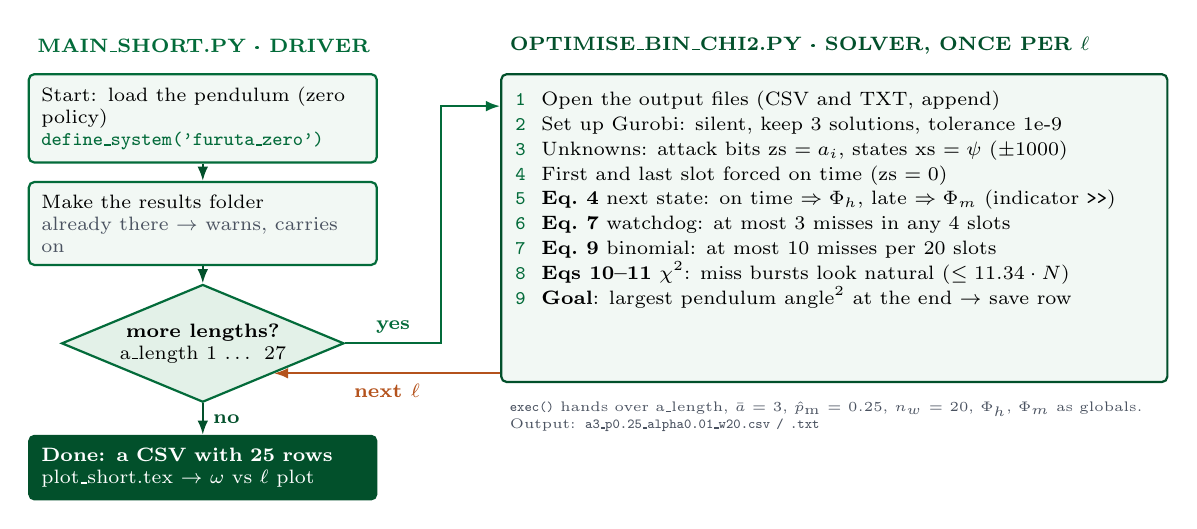
\begin{tikzpicture}[
  fbox/.style={box, text width=4.1cm, minimum height=0.8cm},
]
\node[font=\scriptsize\bfseries, text=mgreen, anchor=west] at (0,0.35) {MAIN\_SHORT.PY \textperiodcentered{} DRIVER};
\node[fbox, anchor=north west] (a) at (0,0) {Start: load the pendulum (zero policy)\\ {\color{mgreen}\ttfamily define\_system('furuta\_zero')}};
\node[fbox, below=0.22cm of a] (b) {Make the results folder\\ {\color{body}already there $\to$ warns, carries on}};
\node[dec, aspect=2.4, font=\scriptsize, below=0.22cm of b] (d) {\textbf{more lengths?}\\a\_length 1 \dots{} 27};
\node[darkbox, text width=4.1cm, minimum height=0.8cm, below=0.4cm of d] (e) {\textbf{Done: a CSV with 25 rows}\\ plot\_short.tex $\to$ $\omega$ vs $\ell$ plot};
\draw[arr] (a) -- (b);
\draw[arr] (b) -- (d);
\draw[arr] (d) -- node[right, font=\scriptsize]{\bfseries no} (e);

\node[font=\scriptsize\bfseries, text=mgreenD, anchor=west] at (6.0,0.35) {OPTIMISE\_BIN\_CHI2.PY \textperiodcentered{} SOLVER, ONCE PER $\ell$};
\node[draw=mgreenD, thick, fill=mgreenXL, rounded corners=2pt, anchor=north west, inner sep=1.8mm, font=\scriptsize] (s) at (6.0,0) {\parbox[t][3.55cm][t]{8.1cm}{%
\renewcommand{\arraystretch}{1.12}%
\begin{tabular}{@{}>{\color{mgreen}\bfseries\ttfamily}l@{\hspace{2mm}}l@{}}
1 & Open the output files (CSV and TXT, append)\\
2 & Set up Gurobi: silent, keep 3 solutions, tolerance 1e-9\\
3 & Unknowns: attack bits zs $=a_i$, states xs $=\psi$ ($\pm$1000)\\
4 & First and last slot forced on time (zs $=0$)\\
5 & \textbf{Eq.~4} next state: on time $\Rightarrow\Phi_h$, late $\Rightarrow\Phi_m$ (indicator \texttt{>>})\\
6 & \textbf{Eq.~7} watchdog: at most 3 misses in any 4 slots\\
7 & \textbf{Eq.~9} binomial: at most 10 misses per 20 slots\\
8 & \textbf{Eqs 10--11} $\chi^2$: miss bursts look natural ($\le 11.34\cdot N$)\\
9 & \textbf{Goal}: largest pendulum angle$^2$ at the end $\to$ save row\\
\end{tabular}}};
\draw[arr, mgreen] (d.east) -- node[above, font=\scriptsize]{\bfseries yes} ($(d.east -| s.west)+(-0.75,0)$) |- ($(s.north west)+(0,-0.42)$);
\draw[arr, accent] (d.south east -| s.west) -- node[below, font=\scriptsize]{\bfseries next $\ell$} (d.south east);
\node[anchor=north west, text width=8.1cm, font=\tiny, text=body, align=left] at ($(s.south west)+(0,-0.12)$) {\texttt{exec()} hands over a\_length, $\bar a=3$, $\hat p_{\mathrm m}=0.25$, $n_w=20$, $\Phi_h$, $\Phi_m$ as globals. Output: \texttt{a3\_p0.25\_alpha0.01\_w20.csv / .txt}};
\end{tikzpicture}
\end{center}
\end{frame}

% =====================================================================
% 5. Part 3: worked example as a decision flow
% =====================================================================
\begin{frame}{Worked example: how one solver call picks the attack}{Part 3 \textperiodcentered{} The code}
\note{One real pass of the loop at a\_length = 7, so attack length 5. The pendulum starts tilted 0.0098 rad. First and last slots are forced hits, leaving 32 possible attacks z1 to z5. Read the decision flow left to right. The watchdog (Eq. 7) removes any attack with 4 misses in a row, for example 0111100, which would do the most damage but would shut the plant down. The binomial test (Eq. 9) allows 10 misses per 20-slot window; with only 5 free slots it cannot bind here. The chi-square test (Eqs 10 to 11, limit 11.34 times N, here 34.0) removes 0111000, because a 3-miss burst is expected only 2 percent of the time (60.3), and 0101010, which is too regular (39.0). Among the survivors the solver maximises the squared angle at step 6: 0110100 wins with chi-square 19.0; its free part 11010 is exactly the sequence printed in Section 5.4.1. The small chart shows why it hurts: without attack the controller pulls the angle 0.0098 to 0.0030; with the attack each miss zeroes the motor command when it was needed, so the angle only reaches 0.0060, twice as far off. Squared: 3.63 against 0.89 times 1e-5, so omega (Def. 5.1) = 2.74e-5, written as CSV row 7.}
\takeaway{a\_length = 7 ($\ell=5$): 32 possible attacks. Three checks remove the risky ones; the most damaging survivor wins.}

\begin{center}
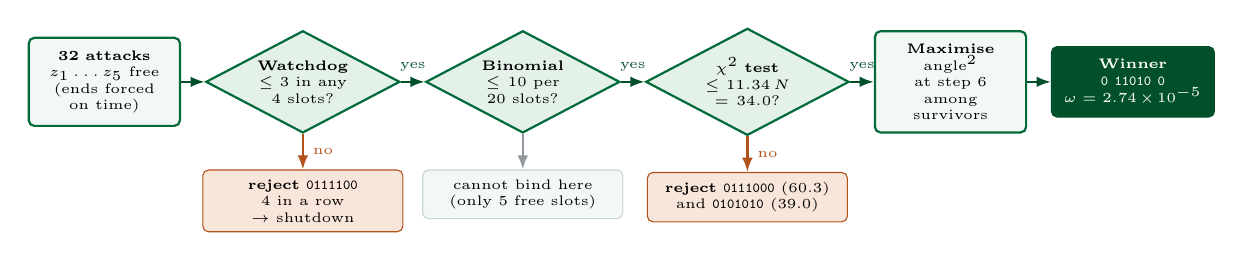
\begin{tikzpicture}[node distance=0.3cm]
\node[box, text width=1.6cm, align=center, font=\tiny] (st) {\textbf{32 attacks}\\$z_1\dots z_5$ free\\(ends forced on time)};
\node[dec, right=of st, text width=1.2cm] (w) {\textbf{Watchdog}\\$\le3$ in any\\4 slots?};
\node[dec, right=of w, text width=1.2cm] (bn) {\textbf{Binomial}\\$\le10$ per\\20 slots?};
\node[dec, right=of bn, text width=1.2cm] (cs) {\textbf{$\chi^2$ test}\\$\le 11.34\,N$\\$=34.0$?};
\node[box, right=of cs, text width=1.6cm, align=center, font=\tiny] (mx) {\textbf{Maximise}\\angle$^2$ at step 6\\among survivors};
\node[darkbox, right=of mx, text width=1.75cm, align=center, font=\tiny] (wn) {\textbf{Winner}\\\texttt{0 11010 0}\\$\omega=2.74\times10^{-5}$};
\draw[arr] (st) -- (w);
\draw[arr] (w) -- node[above, font=\tiny]{yes} (bn);
\draw[arr] (bn) -- node[above, font=\tiny]{yes} (cs);
\draw[arr] (cs) -- node[above, font=\tiny]{yes} (mx);
\draw[arr] (mx) -- (wn);
\node[reject, below=0.45cm of w] (rw) {\textbf{reject} \texttt{0111100}\\4 in a row $\to$ shutdown};
\node[reject, below=0.45cm of bn, draw=rulec, fill=mgreenXL] (rb) {cannot bind here\\(only 5 free slots)};
\node[reject, below=0.45cm of cs] (rc) {\textbf{reject} \texttt{0111000} (60.3)\\and \texttt{0101010} (39.0)};
\draw[arr, accent] (w) -- node[right, font=\tiny]{no} (rw);
\draw[arr, body!60] (bn) -- (rb);
\draw[arr, accent] (cs) -- node[right, font=\tiny]{no} (rc);
\end{tikzpicture}
\end{center}
\vspace{-0.6ex}

\begin{columns}[T,onlytextwidth]
\begin{column}{0.5\textwidth}
{\scriptsize
\renewcommand{\arraystretch}{1.18}\setlength{\tabcolsep}{4pt}
\noindent\begin{tabular}{l l r l}
\rowcolor{mgreen}\color{white}\textbf{Attack} & \color{white}\textbf{Check} & \color{white}\textbf{angle$^2$} & \color{white}\textbf{Result}\\
\rowcolor{mgreenXL}\ttfamily 0000000 & no attack & 0.89 & baseline\\
\rowcolor{mgreenL}\ttfamily 0111100 & 4 in a row & 5.75 & watchdog stop\\
\rowcolor{mgreenXL}\ttfamily 0111000 & $\chi^2$ 60.3 $>$ 34.0 & 4.99 & burst too rare\\
\rowcolor{mgreenL}\ttfamily 0101010 & $\chi^2$ 39.0 $>$ 34.0 & 2.22 & too regular\\
\rowcolor{accentL}\ttfamily\bfseries 0110100 & \textbf{$\chi^2$ 19.0 $\le$ 34.0} & \textbf{3.63} & \textbf{chosen: hidden}\\
\end{tabular}\\[0.3ex]
{\tiny\color{body} angle$^2$ at step 6, in units of $10^{-5}$}}
\end{column}
\begin{column}{0.47\textwidth}
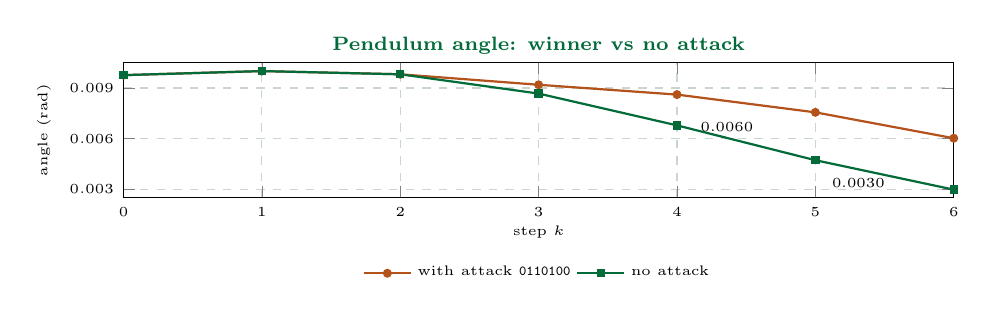
\begin{tikzpicture}
\begin{axis}[
  width=\linewidth, height=3.3cm,
  xmin=0, xmax=6, ymin=0.0025, ymax=0.0105,
  xtick={0,...,6}, ytick={0.003,0.006,0.009},
  yticklabel style={/pgf/number format/fixed,/pgf/number format/precision=3},
  scaled y ticks=false,
  xlabel={step $k$}, ylabel={angle (rad)}, xlabel style={yshift=0.8ex},
  label style={font=\tiny}, tick label style={font=\tiny},
  legend style={font=\tiny, draw=none, fill=none, at={(0.5,-0.42)}, anchor=north}, legend columns=2,
  grid=major, grid style={dashed, rulec},
  title={\scriptsize\bfseries\color{mgreen} Pendulum angle: winner vs no attack}, title style={yshift=-1.5ex},
]
\addplot[accent, thick, mark=*, mark size=1.2pt] coordinates {(0,0.00976)(1,0.01000)(2,0.00981)(3,0.00919)(4,0.00861)(5,0.00756)(6,0.00603)};
\addlegendentry{with attack \texttt{0110100}}
\addplot[mgreen, thick, mark=square*, mark size=1.1pt] coordinates {(0,0.00976)(1,0.01000)(2,0.00981)(3,0.00867)(4,0.00679)(5,0.00473)(6,0.00299)};
\addlegendentry{no attack}
\node[font=\tiny, anchor=west] at (axis cs:4.1,0.0067) {0.0060};
\node[font=\tiny, anchor=west] at (axis cs:5.05,0.0034) {0.0030};
\end{axis}
\end{tikzpicture}
\end{column}
\end{columns}
\end{frame}

% =====================================================================
% 6. Part 3: full result and verification flow
% =====================================================================
\begin{frame}{The full result, checked against the paper}{Part 3 \textperiodcentered{} The code}
\note{Repeating the solver call for all 25 lengths gives the full output of main\_short.py: attack effectiveness omega, the extra squared pendulum angle caused by the attack. The big dot at length 5 is the worked example. Next to it is the matching panel of the paper's Figure 2 (Furuta, a-bar 3); the brown x curve is p-hat 0.25. Same bump near 4, same dip at 7, same peak of about 9.4e-5 at 13, same plateau afterwards. Three regimes: short attacks exploit the initial tilt; the peak interleaves misses and hits (0101101110100); long attacks wait, then strike late (for example 1100000000010110111011010 at length 25). How we checked it, the bottom flow: we could not install Gurobi, so we took the authors' own matrices from define\_system, applied the same constraints, and enumerated every valid 0/1 attack for each length; exhaustive search guarantees the true optimum, and all 25 lengths took about six minutes. The curve and the sequences for lengths 5 and 15 match the paper exactly (Section 5.4.1 quotes them for a-bar 4; identical here because they never use more than three misses in a row). Caveats if asked: main\_short.py does not exit when its results folder exists, so a rerun duplicates rows; a bare except hides failed solves; the free Gurobi licence handles only lengths up to about 10.}
\takeaway{All 25 solver calls together: our reproduced curve has the same shape and peak as the paper's Fig.~2.}

\begin{columns}[T,onlytextwidth]
\begin{column}{0.47\textwidth}
\begin{tikzpicture}
\begin{axis}[
  width=\linewidth, height=4.3cm,
  xmin=1, xmax=25, ymin=0, ymax=11,
  xtick={1,5,10,15,20,25}, ytick={0,5,10},
  xlabel={attack length $\ell$}, ylabel={$\omega$ in $10^{-5}$},
  label style={font=\tiny}, tick label style={font=\tiny},
  grid=major, grid style={dashed, rulec},
  title={\scriptsize\bfseries\color{mgreen} Ours: main\_short.py output}, title style={yshift=-1.5ex},
]
\addplot[accent, thick, mark=*, mark size=1.1pt] table[x=ell, y=omega_e5, col sep=comma] {../../../data/ppt/omega_main_short.csv};
\addplot[only marks, accent, mark=*, mark size=2.4pt] coordinates {(5,2.739) (13,9.450)};
\node[font=\tiny, anchor=west] at (axis cs:13.6,10.1) {\textbf{peak $\ell=13$}};
\node[font=\tiny, anchor=west, align=left] at (axis cs:1.6,7.6) {\textbf{$\ell=5$}: worked\\example (2.74)};
\end{axis}
\end{tikzpicture}
\end{column}
\begin{column}{0.22\textwidth}
\centering
{\scriptsize\bfseries\color{mgreen} Paper, Fig.~2 ($\bar a=3$)}\\[0.6ex]
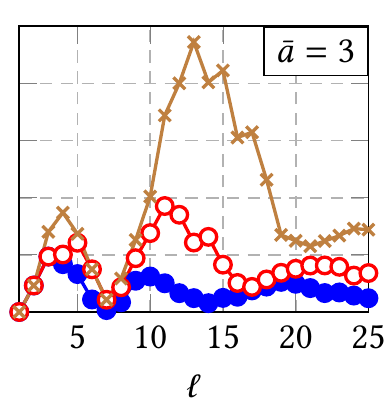
\includegraphics[width=\linewidth]{../../assets/abhishek/paper_fig2_a3.png}\\[0.4ex]
{\tiny\color{body} brown $\times$ = \phatm{} 0.25}
\end{column}
\begin{column}{0.27\textwidth}
\begin{block}{What the curve shows}
\textbf{Short} attacks exploit the initial tilt (bump at $\ell\approx4$)\\[0.4ex]
\textbf{Peak} at $\ell=13$: misses interleaved with hits\\[0.4ex]
\textbf{Long} attacks wait, then strike late
\end{block}
\begin{block}{Matches the paper}
same bump, dip and peak; $\ell=5$ and $\ell=15$ sequences identical to \S5.4.1
\end{block}
\end{column}
\end{columns}

\vspace{0.6ex}
{\scriptsize\bfseries\color{mgreen} How we reproduced it without Gurobi}\\[0.3ex]

\begin{tikzpicture}[node distance=0.4cm]
\node[pill, text width=2.95cm] (v1) {Authors' matrices\\[-1pt]{\normalfont\ttfamily define\_system()}};
\node[pill, text width=2.95cm, right=of v1] (v2) {Same constraints\\[-1pt]{\normalfont Eqs 7, 9, 10--11}};
\node[pill, text width=2.95cm, right=of v2] (v3) {Try every valid attack\\[-1pt]{\normalfont $\ell=1\dots25$, $\sim$6 min}};
\node[pill, text width=2.95cm, right=of v3, fill=mgreen, text=white] (v4) {Same curve as Fig.~2\\[-1pt]{\normalfont guaranteed optimum}};
\draw[arr] (v1) -- (v2); \draw[arr] (v2) -- (v3); \draw[arr] (v3) -- (v4);
\end{tikzpicture}
\end{frame}

\end{document}
